\subsection{Judge accuracy in the two regimes (O2)}
\label{sec:res-acc}

\Cref{tab:main} and \cref{fig:regimes} report pairwise accuracy.  With the
\CJB{} protocol (mean of both presentation orders), every judge is close to the
50\% random baseline in \emph{both} regimes: \AccRangeC{} on the single-file
control subset and \AccRangeR{} on \RJB{}.  The confidence intervals of all
judges include or lie below 50\% on \RJB{}.  For the small judges this is
consistent with the base paper, which reports that even large non-thinking
judges stay below 60\% on \CJB{}.  The regime comparison is therefore
dominated by a floor effect for raw accuracy; it becomes informative only after
removing position bias, below.

\begin{figure}[t]
\centering
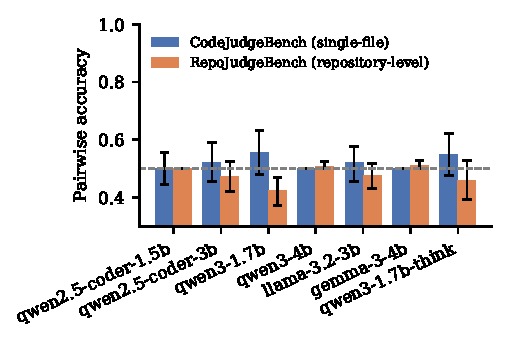
\includegraphics[width=\columnwidth]{../results/figures/regimes.pdf}
\caption{Pairwise accuracy of each judge on the \CJB{} control subset and on
\RJB{} (95\% bootstrap CIs). The dashed line is the random baseline.}
\label{fig:regimes}
\end{figure}

\begin{table*}[t]
\caption{Pairwise accuracy (\%) with 95\% bootstrap CIs on the \CJB{} control subset (single-file) and on \RJB{} (repository-level, diff-only); a pair's accuracy is the mean of its two presentation orders. $\Delta$ = control $-$ \RJB{}. \emph{Calibrated} = accuracy after balanced position calibration (the probability given to the gold patch is averaged over both orders before deciding). Random = 50\%; the execution oracle scores 0\% on \RJB{} by construction.}
\label{tab:main}
\centering\footnotesize
\begin{tabular}{@{}lllrrlr@{}}
\toprule
 & \multicolumn{2}{c}{Accuracy} & & \multicolumn{2}{c}{Calibrated accuracy} & \\
\cmidrule(lr){2-3}\cmidrule(lr){5-6}
Judge & \CJB{} control & \RJB{} & $\Delta$ & \CJB{} & \RJB{} & $n$ (pairs) \\
\midrule
Qwen2.5-Coder-1.5B & 50.0 [44, 56] & -- & -- & 55.6 & -- & 45/-- \\
Qwen3-1.7B & 57.1 [45, 69] & -- & -- & 76.2 & -- & 21/-- \\
\bottomrule
\end{tabular}
\end{table*}


\subsection{Position bias and self-consistency (O5)}
\label{sec:res-robust}

\Cref{tab:robust} shows why raw accuracy is uninformative: the verdicts are
dominated by the \emph{slot} in which a patch is shown.  \RobustText{}
Self-consistency (SC) is high exactly where a judge is most position-biased, so
consistency across samples is not evidence of reliability.

\begin{table*}[t]
\caption{Robustness (O5), control (C) vs.\ \RJB{} (R), in \%. \emph{Pos.\ gap}: accuracy with the gold patch shown first minus shown second. \emph{Flip}: share of pairs whose verdict selects the same slot in both orders. $P(A)$: mean probability of choosing the first slot. \emph{SC}: expected agreement of two independent $T{=}1$ samples of the verdict.}
\label{tab:robust}
\centering\footnotesize
\begin{tabular}{@{}lrrrrrrrr@{}}
\toprule
 & \multicolumn{2}{c}{Pos.\ gap} & \multicolumn{2}{c}{Flip} & \multicolumn{2}{c}{$P(A)$} & \multicolumn{2}{c}{SC} \\
\cmidrule(lr){2-3}\cmidrule(lr){4-5}\cmidrule(lr){6-7}\cmidrule(lr){8-9}
Judge & C & R & C & R & C & R & C & R \\
\midrule
Qwen2.5-Coder-1.5B & -24.4 & -- & 86.7 & -- & 48.5 & -- & 50.5 & -- \\
Qwen3-1.7B & -38.1 & -- & 66.7 & -- & 36.3 & -- & 68.9 & -- \\
\bottomrule
\end{tabular}
\end{table*}


\textbf{Balanced position calibration.}  Averaging the probability assigned to
the gold patch over both orders removes a constant slot preference
(\cref{tab:main}, ``Calibrated'').  \CalibText{}

\subsection{Length bias}
\label{sec:res-length}

The variant differs from the gold patch by a single mutation, but the mutation
changes the size of the diff: in \VarLongerShare{} of judged pairs the
defective variant's diff is longer (e.g.\ unwrapping a \texttt{with} block
re-indents its body).  \Cref{tab:length} shows that judge preferences follow
this length difference.  \LengthText{}  The same artefact makes the benchmark
exploitable: choosing the patch with fewer changed lines scores
\LengthHeurAcc{} (\cref{tab:baselines}).  We report this as a limitation of the
current construction and as a warning for execution-free judges, which can
look competent on benchmarks whose negatives are systematically longer or
shorter than the positives.

\begin{table}[t]
\caption{Length bias on \RJB{}: position-calibrated accuracy (\%) by whether the defective variant's diff has more, the same or fewer changed lines than the gold patch (judged pairs: 112 / 24 / 19); $n$ in parentheses. Last column: share of pairs of unequal length in which the judge prefers the longer patch.}
\label{tab:length}
\centering\footnotesize
\begin{tabular}{@{}lrrrl@{}}
\toprule
Judge & Var.\ longer & Same & Var.\ shorter & Prefers longer \\
\midrule
Qwen2.5-Coder-1.5B & 19.5 (77) & 37.5 (16) & 72.7 (11) & 79.5 [72, 87] \\
Qwen2.5-Coder-3B & 11.5 (26) & 42.9 (7) & 75.0 (4) & 86.7 [74, 97] \\
Qwen3-1.7B & 22.0 (59) & 53.8 (13) & 71.4 (7) & 77.3 [66, 88] \\
Qwen3-4B & 66.0 (47) & 55.6 (9) & 85.7 (7) & 40.7 [27, 55] \\
Llama-3.2-3B & 40.5 (74) & 93.3 (15) & 91.7 (12) & 64.0 [53, 75] \\
Gemma-3-4B & 62.5 (64) & 42.9 (14) & 60.0 (10) & 40.5 [30, 52] \\
Qwen3-1.7B-think & 26.9 (26) & 71.4 (7) & 50.0 (4) & 70.0 [52, 88] \\
All judges & 37.3 (373) & 56.8 (81) & 74.5 (55) & 64.3 [59, 69] \\
\bottomrule
\end{tabular}
\end{table}


\subsection{Degradation with diff size (O3)}
\label{sec:res-scaling}

\Cref{fig:scaling} bins accuracy by the size of the gold patch and
\cref{tab:scaling} reports the pooled logistic regression.  \ScalingText{}

\begin{figure}[t]
\centering
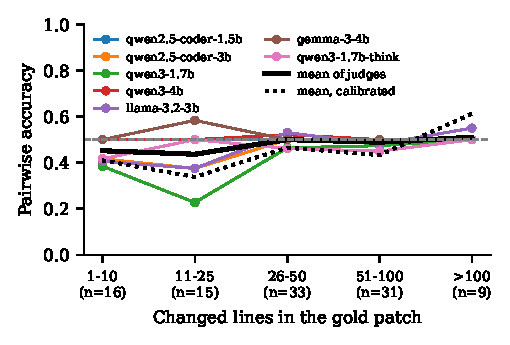
\includegraphics[width=\columnwidth]{../results/figures/scaling.pdf}
\caption{Accuracy by gold-patch size (changed lines); bin sizes in parentheses.
The dotted line is the judges' mean after position calibration.}
\label{fig:scaling}
\end{figure}

\begin{table}[t]
\caption{Logistic regression of per-presentation correctness on diff size (pooled over judges; 1018 presentations of 509 judge--pair combinations; SEs clustered by pair).}
\label{tab:scaling}
\centering\footnotesize
\begin{tabular}{@{}lrrr@{}}
\toprule
Predictor & $\beta$ & 95\% CI & $p$ \\
\midrule
Intercept & -0.389 & [-0.714, -0.065] & 0.019 \\
$\log_2$ changed lines & +0.058 & [-0.006, +0.121] & 0.074 \\
Files touched & -0.024 & [-0.055, +0.007] & 0.129 \\
Hunks & +0.015 & [-0.005, +0.036] & 0.147 \\
\bottomrule
\end{tabular}
\end{table}


\subsection{Defect-class error profile (O4)}
\label{sec:res-classes}

\Cref{tab:classes} breaks accuracy down by class.  \ClassText{}

\begin{table*}[t]
\caption{Accuracy (\%) by defect class on \RJB{} (diff-only). The pooled row averages pairs over all judges and reports a bootstrap CI.}
\label{tab:classes}
\centering\footnotesize
\begin{tabular}{@{}lrrrrr@{}}
\toprule
Judge & N+1 query & Race / concurrency & Authorisation & Resource leak & Error swallowing \\
\midrule
Qwen2.5-Coder-1.5B & 50.0 & 50.0 & 50.0 & 50.0 & 50.0 \\
Qwen2.5-Coder-3B & -- & 50.0 & 50.0 & 50.0 & 46.6 \\
Qwen3-1.7B & 50.0 & 50.0 & 50.0 & 40.0 & 41.5 \\
Qwen3-4B & -- & 50.0 & 50.0 & 50.0 & 51.1 \\
Llama-3.2-3B & 50.0 & 50.0 & 50.0 & 40.6 & 48.7 \\
Gemma-3-4B & 50.0 & 50.0 & 50.0 & 50.0 & 51.5 \\
Qwen3-1.7B-think & -- & 50.0 & 50.0 & 50.0 & 44.8 \\
\midrule
All judges & 50.0 [50, 50] & 50.0 [36, 61] & 50.0 [50, 50] & 46.6 [43, 50] & 48.2 [46, 50] \\
Pairs ($n$) & 2 & 5 & 5 & 25 & 118 \\
Static (relevant) & 50.0 & 50.0 & 50.0 & 66.7 & 70.8 \\
Static (all rules) & 75.0 & 28.6 & 10.0 & 47.0 & 53.0 \\
\bottomrule
\end{tabular}
\end{table*}


\subsection{Mitigation: repository context, and thinking (O6)}
\label{sec:res-context}

\Cref{tab:context} compares context-augmented prompts with the diff-only
prompt on the same pairs.  \ContextText{}

\begin{table*}[t]
\caption{Mitigation (O6) and thinking: accuracy (\%) of each condition and paired difference to the diff-only prompt on the same pairs (raw and after balanced position calibration).}
\label{tab:context}
\centering\footnotesize
\setlength{\tabcolsep}{3pt}
\begin{tabular}{@{}llrrrr@{}}
\toprule
Judge & Condition & Acc. & $\Delta$ & $\Delta$ calib. & $n$ \\
\midrule
Qwen2.5-Coder-1.5B & + file, 6k chars & 50.0 & +0.0 [-3, 3] & +11.1 [-2, 26] & 45 \\
Qwen2.5-Coder-1.5B & + retrieved, 2k chars & 50.0 & +0.0 [-2, 2] & +6.7 [-5, 20] & 60 \\
Qwen2.5-Coder-1.5B & + retrieved, 6k chars & 49.2 & -0.8 [-4, 2] & +10.0 [-3, 23] & 60 \\
Qwen3-1.7B & + retrieved, 6k chars & 47.3 & +5.4 [-4, 15] & +21.6 [5, 40] & 37 \\
Qwen3-1.7B & thinking & 45.9 & +4.1 [-4, 13] & +16.2 [3, 32] & 37 \\
\bottomrule
\end{tabular}
\end{table*}


\subsection{Baselines and point-wise judging}
\label{sec:res-baselines}

\Cref{tab:baselines} lists the non-LLM baselines.  \BaselineText{}

\begin{table}[t]
\caption{Non-LLM baselines and point-wise judging on \RJB{} (accuracy, \%).}
\label{tab:baselines}
\centering\footnotesize
\begin{tabular}{@{}lrl@{}}
\toprule
Method & Acc. & Notes \\
\midrule
Random & 50.0 & -- \\
Execution oracle (PR tests) & 0.0 & by construction \\
Static analysis, relevant rules & 60.0 & [50, 70]; flags variant 20.0\%, gold 0.0\% \\
Static analysis, all rules & 43.3 & [23, 63]; flags variant 33.3\%, gold 46.7\% \\
\bottomrule
\end{tabular}
\end{table}

